\chapter{\label{ch:intro} Introduction}

The use of Augmented Reality (AR) in robotic systems has seen a rise in the last decade, This project aims to develop an AR system for a wheeled robot, which should enhance its functionality and provide an overall better user experience. This project builds upon previous work in robotics and aims to integrate AR technology to improve he human-machine experience.

%@@@@@@@@@@@@@@@@@@@@@@@@@@@@@@@@@@@@@@@@@@@@@@@@@@@@@@@@@@@@@@@@@@@@@@@@@@@@@@@@@@@@@@@@@@@@@@@@@@@@@@
\section{\label{sec:backg}Background}
The concept of autonomous vehicles dates back to Leonardo Da Vinci's 16th-century designs, although practical implementations only emerged in the 1980s \cite{Mobileye2023}. Radio-controlled (RC) cars, introduced earlier by Elettronica \cite{RC_Crush2023}, evolved from combustion engines to electric motors, expanding their applications across various industries \cite{GoogleBooks2017}.
\begin{figure}[h]
\centering
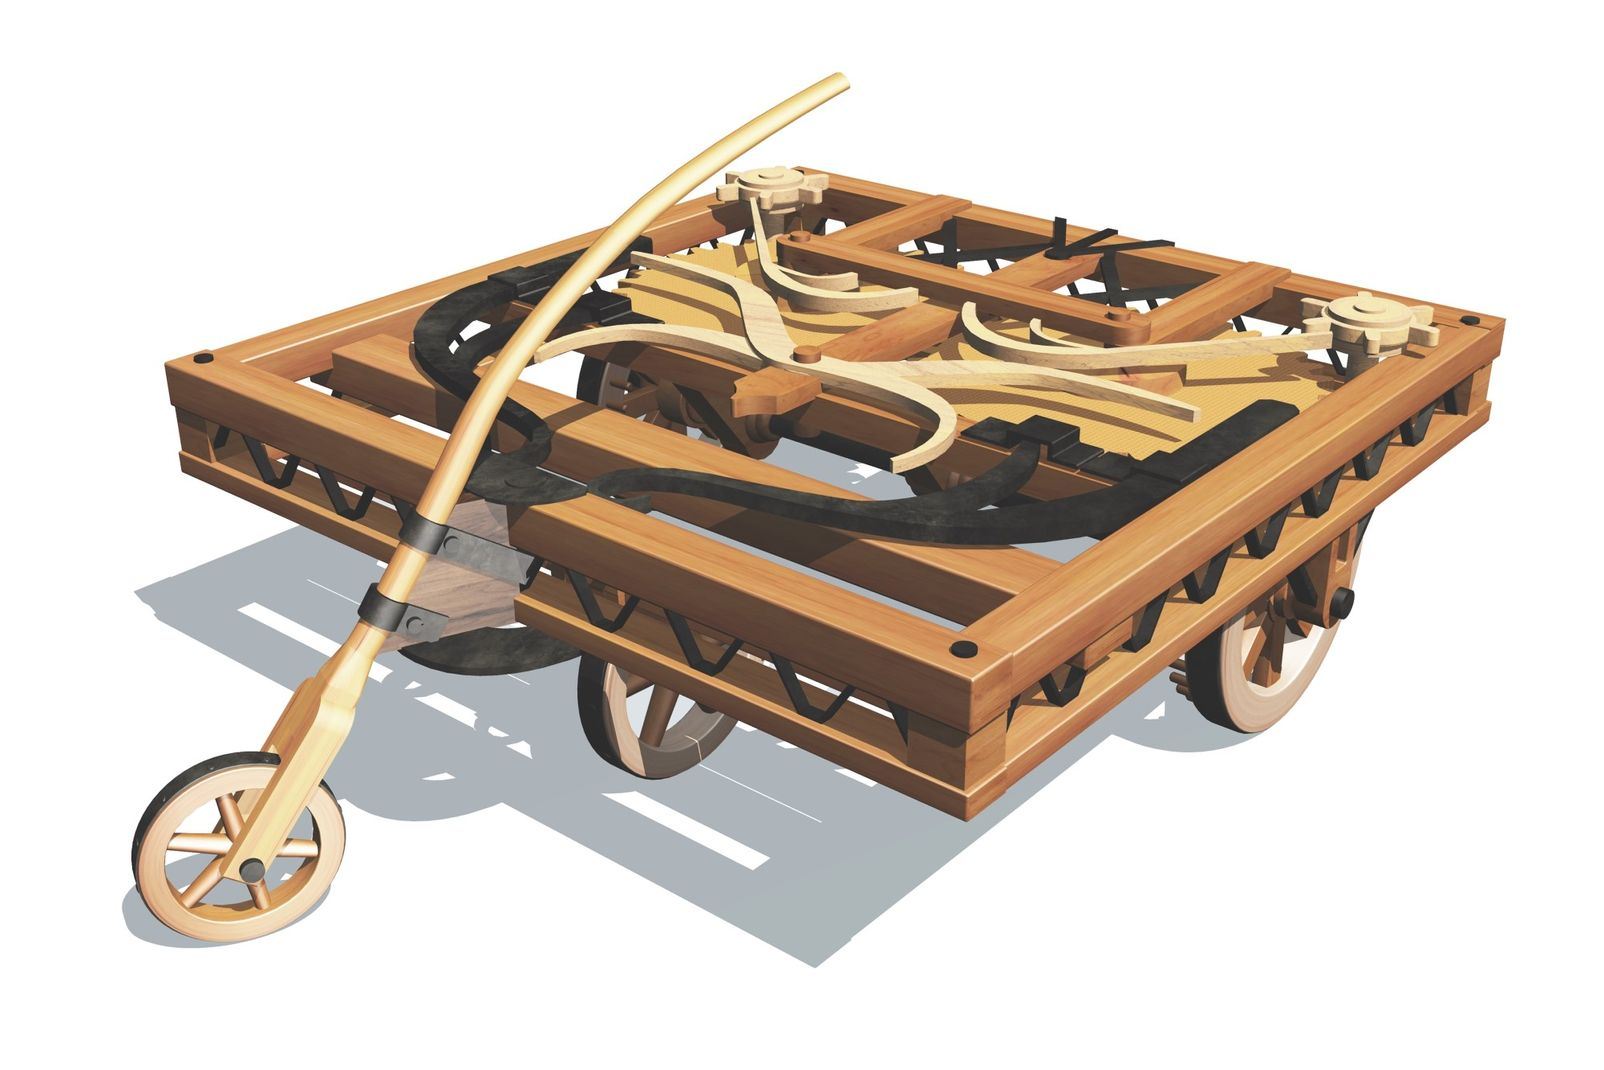
\includegraphics[width=0.35\textwidth]{ch1/figs/Vinci_car.jpg}
\caption{Model of autonomous car designed by Leonardo Da Vinci}
\label{fig:davinci_car}
\end{figure}
As we approach the Fifth Industrial Revolution (5IR), the focus shifts to a symbiotic relationship between humans and AI-powered robots, emphasizing workplace efficiency while maintaining a human-centric approach \cite{Samuels2023}. Augmented Reality (AR) plays a crucial role in this evolution, bridging the gap between humans and machines in areas such as manufacturing, healthcare, and human-robot interaction (HRI) \cite{Dalle2021}.

In the context of autonomous systems, fiducial markers (e.g., ARToolKit, AprilTags, ArUco) have become integral to robotics and AR applications. These markers facilitate robot navigation, environmental mapping, and interaction zone definition. The choice of marker system depends on specific application requirements, available computational resources, and desired accuracy.

The integration of AR and fiducial markers in robotics enhances perception, navigation, and interaction capabilities, pushing the boundaries of human-robot collaboration and making autonomous robots more adaptable and intelligent.





%@@@@@@@@@@@@@@@@@@@@@@@@@@@@@@@@@@@@@@@@@@@@@@@@@@@@@@@@@@@@@@@@@@@@@@@@@@@@@@@@@@@@@@@@@@@@@@@@@@@@@@
\section{\label{sec:probdesc}Problem Description}

As robots continue to evolve with so does our demand for more intuitive and seamless interaction with these robots. Traditional control methods often fall short when it comes to offering the flexibility and situational awareness needed to integrate robots effectively into dynamic, real-world environments. This project addresses several key challenges in the domain of mobile robot control and environmental interaction:

\begin{enumerate}
    \item \textbf{Limited Contextual Awareness}: Current remote-controlled robots often operate with minimal understanding of their surroundings, leading to inefficient navigation and potential safety hazards in complex environments.
    \item \textbf{Inflexible Control Mechanisms}: Many existing robot control systems rely on fixed command sets that do not adapt to changing environmental conditions or task requirements, limiting their versatility and usability.
    \item \textbf{Lack of Intuitive Feedback}: Users often struggle to interpret the robot's status, intentions, or responses to environmental stimuli, creating a communication gap between the human operator and the robotic system.
    \item \textbf{Absence of Dynamic Task Assignment}: Most mobile robots are pre-programmed for specific tasks and lack the ability to receive and interpret new instructions or environmental cues on the fly.
    \item \textbf{Integration Challenges}: Incorporating augmented reality (AR) elements into robotic systems presents technical challenges in terms of real-time processing, accurate marker detection, and seamless information overlay.
\end{enumerate}


%@@@@@@@@@@@@@@@@@@@@@@@@@@@@@@@@@@@@@@@@@@@@@@@@@@@@@@@@@@@@@@@@@@@@@@@@@@@@@@@@@@@@@@@@@@@@@@@@@@@@@@
%\section{\label{sec:focus}Focus}

%@@@@@@@@@@@@@@@@@@@@@@@@@@@@@@@@@@@@@@@@@@@@@@@@@@@@@@@@@@@@@@@@@@@@@@@@@@@@@@@@@@@@@@@@@@@@@@@@@@@@@@
\section{\label{sec:objectives}Objectives}

The primary objective of this project is to enhance human-robot interaction (HRI) by integrating Augmented Reality (AR) technology with mobile robotics. Leveraging AR and visual markers like ArUco codes, the robot will be able to navigate and perform tasks in a more interactive, intuitive, and human-centered manner, thus improving the overall user experience. This project focuses on providing the human operator with an augmented view of the environment and enhancing the robot’s context-awareness to better perform dynamic, real-time tasks.

More specifically, the project seeks to develop a control system that facilitates dynamic, visual-based communication between a human user and the robot. By augmenting the environment with visual markers and AR interfaces, the robot will better understand its surroundings and perform context-aware tasks. Different "control zones" will trigger specific robot behaviors based on the visual markers detected by its camera, providing real-time feedback through AR-enhanced visualizations.

\subsection{Main Objectives}
\begin{enumerate}
    \item \textbf{Development of Control Zones}: AR-based control zones will guide the robot’s behavior. These zones will define parameters such as speed adjustments, task initiation, and areas where the robot must stop or change direction based on AR markers.
    \item \textbf{Integration of Dynamic Instructions}: Using ArUco markers, the robot will receive real-time commands to perform various tasks, including navigation, task execution, and environment-specific instructions triggered by marker detection.
    \item \textbf{Environmental Mapping and Task Interaction}: The robot will use visual markers to create a simple map of its surroundings, enabling it to track landmarks, avoid obstacles, and interact with specific objects in its environment.
    \item \textbf{Improving User Engagement}: AR technology will allow users to visually instruct and monitor the robot’s progress in real-time, offering a more interactive and immersive user experience that enhances both usability and functionality.
\end{enumerate}

\subsection{Secondary Objectives}

In addition to the main objectives, the project will explore two secondary automated functionalities to improve robot autonomy:
\begin{enumerate}
    \item \textbf{Object Avoidance}: The robot will recognize specific markers (e.g., a warning cone) and avoid coming within a defined distance (e.g., 20cm) of those objects. This feature will prevent the robot from advancing if it is too close to an obstacle, even if the human operator continues pressing forward.
    \item \textbf{Wheel Slip Detection}: The robot will detect terrain changes that could cause wheel slip, such as transitioning from solid ground to a slippery surface. Instead of relying on wheel rotation counters, the robot will monitor power draw characteristics to detect traction issues and adjust accordingly.
\end{enumerate}


These enhancements aim to address the current limitations in HRI by making robot control more intuitive and responsive in dynamic environments. They also contribute to the broader goal of improving human-robot collaboration in both industrial and everyday contexts, creating a seamless and human-centered interaction model.


\section{\label{sec:terms}Terms of Reference}

This project aims to enhance human-robot interaction (HRI) by integrating Augmented Reality (AR) into a mobile robot. The system requirements, established through research, discussions with the supervisor, and analysis of the intended user environment, guide both the technical implementation and user experience. Key requirements include operating in AR-defined control zones, integrating dynamic instructions based on ArUco marker detection, environmental mapping using visual markers, providing real-time visual feedback, implementing object avoidance functionality, and detecting wheel slip events.

To meet these requirements, the system will implement several functionalities, including AR-based control zones, real-time ArUco marker processing, visual marker-based environmental mapping and obstacle avoidance, AR-based visual feedback for operators, object avoidance behavior, and wheel slip detection. Testing procedures have been outlined to ensure the system meets these requirements and functionalities, with specific sub-tests designed to check each function and requirement individually.

%\section{\label{sec:methology_overview}Methodology Overview}

\section{\label{sec:scope}Scope and Limitations}

This project was conducted under several significant constraints that shaped the scope of the research and development process. These constraints were primarily due to limitations in time, budget, and available resources, which directly impacted the scale of the implementation and the range of features that could be developed.

The project had a total budget of R2000, which restricted the procurement of high-end components and forced the use of readily available, cost-effective hardware. Additionally, the project timeline was set at three months, limiting the ability to explore more advanced functionalities and requiring a focused approach to key objectives. These constraints influenced both the design and testing phases of the project.

Furthermore, ethical considerations were taken into account, particularly in ensuring that no invasive or harmful testing methods were used. The project did not involve human or animal subjects, which helped to avoid potential ethical conflicts and the need for additional approvals.

\begin{itemize}
    \item \textbf{Time constraints:} The project had a strict timeline of three months, which limited the scope of research, prototyping, and testing phases. This required prioritizing key functionalities over more exploratory objectives.
    \item \textbf{Budget limitations:} With a budget of R2000, cost-effective hardware and software solutions had to be utilized, which influenced decisions on components such as sensors, markers, and AR technology. High-end equipment was not feasible.
    \item \textbf{Technical scope:} The project focused on AR integration for basic control and task interaction but did not include advanced machine learning algorithms or high-level autonomy features due to time and resource constraints.
    \item \textbf{Ethical limitations:} The project did not involve any human or animal subjects, thereby avoiding potential ethical conflicts. All testing was performed in controlled environments using non-invasive methods.
    \item \textbf{Environmental considerations:} The robot was tested in a limited set of predefined environments due to time and budget constraints. Broader testing in varying environments or larger spaces was outside the scope of this project.
\end{itemize}

Despite these limitations, the project successfully demonstrated the integration of AR in human-robot interaction. While the constraints limited the full realization of more advanced features, the focused approach allowed the core objectives to be met within the available resources and timeline. Further development could build upon this foundation to explore more complex functionalities and broader applications.


\section{\label{sec:plan_of_development}Plan of Development}

This thesis is structured into six chapters, each focusing on different aspects of the research and development process. The chapters build upon each other to present a coherent narrative from the conceptual framework to the implementation, testing, and conclusions of the project.

\textbf{Chapter 2: Literature Review}

Chapter 2 discusses the foundational technologies, theories, and techniques that underpin this project. It provides an overview of the state of the art in human-robot interaction (HRI), mobile robotics, and the use of Augmented Reality (AR) in robotics. This chapter will also review key research papers and methodologies that are relevant to the design and implementation of AR-enhanced control systems.

\textbf{Chapter 3: Methodology}

Chapter 3 presents the research methodology used for this project. It provides detailed explanations of the procedures, experimental setups, and tools used for the development and testing of the system. In particular, the acceptance tests will be discussed, outlining how each item of functionality and requirement will be meticulously validated through controlled tests. The methodology will emphasize how these tests demonstrate the satisfaction of both functional and system requirements.

\textbf{Chapter 4: Prototype Design}

Chapter 4 focuses on the design of the system. It provides details on the hardware and software design choices, discussing how the various subsystems (e.g., AR integration, control zones, and dynamic instructions) were conceived and implemented. For a prototype-based approach, this chapter will also describe the physical setup, robot design, and any relevant architectural decisions. Visuals such as diagrams, screenshots, and code snippets will be used to illustrate key design elements.

\textbf{Chapter 5: Results and Analysis}

Chapter 5 presents the results obtained from the system tests. These results will showcase how the robot interacted with AR markers and control zones, as well as its performance in dynamic environments. Data from the acceptance tests will be analyzed to assess the system’s functionality and its success in meeting the project’s objectives. This chapter will also include observations on the system's performance, its limitations, and any issues encountered during testing.

\textbf{Chapter 6: Discussion and Conclusion}

Chapter 6 concludes the thesis by reflecting on the overall project, summarizing the key findings, and discussing the implications of the results. It will cover the challenges faced during the project, how they were addressed, and potential areas for improvement. This chapter will also discuss future work, proposing possible enhancements and directions for further research to extend the project’s scope and applications.

\textbf{References}

Finally, all cited works, including books, journal articles, conference papers, and other relevant sources, will be compiled in the References section according to the appropriate referencing style.

